\let\negmedspace\undefined
\let\negthickspace\undefined
\documentclass[journal]{IEEEtran}
\usepackage[a5paper, margin=10mm, onecolumn]{geometry}
%\usepackage{lmodern} % Ensure lmodern is loaded for pdflatex
% \usepackage{tfrupee} % Include tfrupee package

\setlength{\headheight}{1cm} % Set the height of the header box
\setlength{\headsep}{0mm}     % Set the distance between the header box and the top of the text

\usepackage{gvv-book}
\usepackage{gvv}
\usepackage{cite}
\usepackage{amsmath,amssymb,amsfonts,amsthm}
\usepackage{algorithm}
\usepackage{algorithmic}
\usepackage{graphicx}
\usepackage{textcomp}
\usepackage{xcolor}
\usepackage{txfonts}
\usepackage{listings}
\usepackage{enumitem}
\usepackage{mathtools}
\usepackage{gensymb}
\usepackage{comment}
\usepackage[breaklinks=true]{hyperref}
\usepackage{tkz-euclide} 
\usepackage{listings}
% \usepackage{gvv}                                        
\def\inputGnumericTable{}                                 
\usepackage[latin1]{inputenc}                                
\usepackage{color}                                            
\usepackage{array}                                            
\usepackage{longtable}                
\usepackage{calc}                                             
\usepackage{multirow}                                         
\usepackage{hhline}                                           
\usepackage{ifthen}                             
\usepackage{caption}              
\usepackage{lscape}
\usepackage{subcaption}
\usepackage{circuitikz}
\captionsetup{compatibility=false}
% \captionsetup{compactibility=false}
% \usepackage{algpseudocode}
\begin{document}

\bibliographystyle{IEEEtran}
\vspace{3cm}

\title{Experiment 4} 
\author{S A Aravind Eswar and Eshan Sharma}
{\let\newpage\relax\maketitle}

\section{Aim}

To study and analyze the transient response of an LC circuit, determine the natural frequency (\(\Omega_n\)), and calculate the damping ratio (\(\xi\)) using theoretical and experimental methods.

\section{Materials and Apparatus Required}

\begin{enumerate}
	\item 100 $\mu$F Capacitor
	\item Largest available inductor in the lab (denoted as \(L\))
	\item Resistor (small value for practical considerations)
	\item DC Power Supply
	\item Oscilloscope
\end{enumerate}

\section{Theory}

An LC circuit consists of an inductor (\(L\)) and a capacitor (\(C\)) connected in parallel. When a charged capacitor is connected to an inductor, energy oscillates between the capacitor's electric field and the inductor's magnetic field. This oscillatory behavior is governed by the second-order differential equation:
\[
L \frac{d^2q}{dt^2} + R \frac{dq}{dt}+\frac{q}{C} = 0,
\]
where \(q(t)\) is the charge on the capacitor as a function of time.

The natural frequency of oscillation is given by:
\[
\omega_n = \frac{1}{\sqrt{LC}},
\]
where:
- \(L\) is the inductance in henries (H),
- \(C\) is the capacitance in farads (F).

For an ideal LC circuit (no resistance), the damping ratio (\(\xi = 0\)) indicates purely oscillatory behavior. However, in practical circuits, resistance (\(R\)) introduces damping, and the damping ratio becomes:
\[
\xi = \frac{R}{2} \sqrt{\frac{C}{L}}.
\]

From this, we get,

\begin{align*}
    \omega = \omega_n \sqrt{1 - \xi^2 }
\end{align*}

where, $\omega$ is the oscillating frequency 

\begin{figure}[!ht]
	\centering
	\resizebox{0.6\textwidth}{!}{
		\begin{circuitikz}
			\tikzstyle{every node}=[font=\LARGE]
			\draw (10.5,13) to[R] (10.5,11.25);
			\draw (12.25,14) to[L ] (14.25,14);
			\draw (15.75,13) to[C] (15.75,11.25);
			\draw (10.5,13) to[short] (10.5,14);
			\draw (10.5,14) to[short] (12.25,14);
			\draw (14.25,14) to[short] (15.75,14);
			\draw (15.75,14) to[short] (15.75,13);
			\draw (10.5,10.25) to[short] (15.75,10.25);
			\draw (15.75,11.25) to[short] (15.75,10.25);
			\draw (10.5,11.25) to[short] (10.5,10.25);
			\node [font=\LARGE] at (11,11.5) {$+$};
			\node [font=\LARGE] at (12.5,14.25) {$+$};
			\node [font=\LARGE] at (15.5,11.5) {$+$};
			\node [font=\LARGE] at (14,14.25) {$-$};
			\node [font=\LARGE] at (15.5,12.75) {$-$};
			\node [font=\LARGE] at (11,12.75) {$-$};
			\draw [->, >=Stealth] (12.5,11.75) .. controls (12.25,12.75) and (14,13) .. (13.75,11.75) ;
			\node [font=\LARGE] at (13,11.75) {i};
		\end{circuitikz}
	}
	\label{fig:LC circuit with internal resistance}
	
\end{figure}


For experimental analysis, we monitor voltage waveforms using an oscilloscope. The observed oscillation frequency can be compared with theoretical calculations to validate the model.

\section{Procedure}

\begin{enumerate}
	\item Precharge the Capacitor:
	\begin{itemize}
		\item Connect the capacitor to a 5V DC power supply.
		\item Once charged, disconnect it carefully without discharging.
	\end{itemize}
	
	\item Construct the LC Circuit:
	\begin{itemize}
		\item Connect the charged capacitor in parallel with the largest available inductor.
		\item Ensure minimal resistance in wiring.
	\end{itemize}
	
	\item Capture Transient Response:
	\begin{itemize}
		\item Use an oscilloscope to monitor voltage across the capacitor.
		\item Observe natural oscillations.
	\end{itemize}
	
	\item Calculate Theoretical Values:
	\begin{itemize}
		\item Compute natural frequency (\(\Omega_n = 1/\sqrt{LC}\)).
		\item Estimate damping ratio (\(\xi = R/2\sqrt{\frac{C}{L}}\)) if resistance is non-negligible.
	\end{itemize}
	
	\item Compare with Experimental Results:
	\begin{itemize}
		\item Extract oscillation frequency from oscilloscope data.
		\item Compare with theoretical calculations.
	\end{itemize}

	
\end{enumerate}

\section{Observations}

We use $1nF$ capacitor with a $2.2mH$ inductor. This gives,
\begin{align*}
    \omega_n = \frac{1}{\sqrt{LC}} = 9.94053\times 10^{5} rad/s
\end{align*}

Given,$10\%$ error in $L$, and $20\%$ error in $C$,

Tolerance is given by,

\begin{align*}
	\frac{\Delta \omega_n}{\omega_n} &= \frac{1}{2}\left(\frac{\Delta L}{L} + \frac{\Delta C}{C}\right)\\
	\frac{\Delta\omega_n}{\omega_n} &= 0.15 
\end{align*}

Giving us a tolerance of $15\%$

\begin{align*}
	\omega_n = (9.94 \pm 1.49) \times 10^5 rad/s
\end{align*}

\begin{figure}[h]
	\centering
	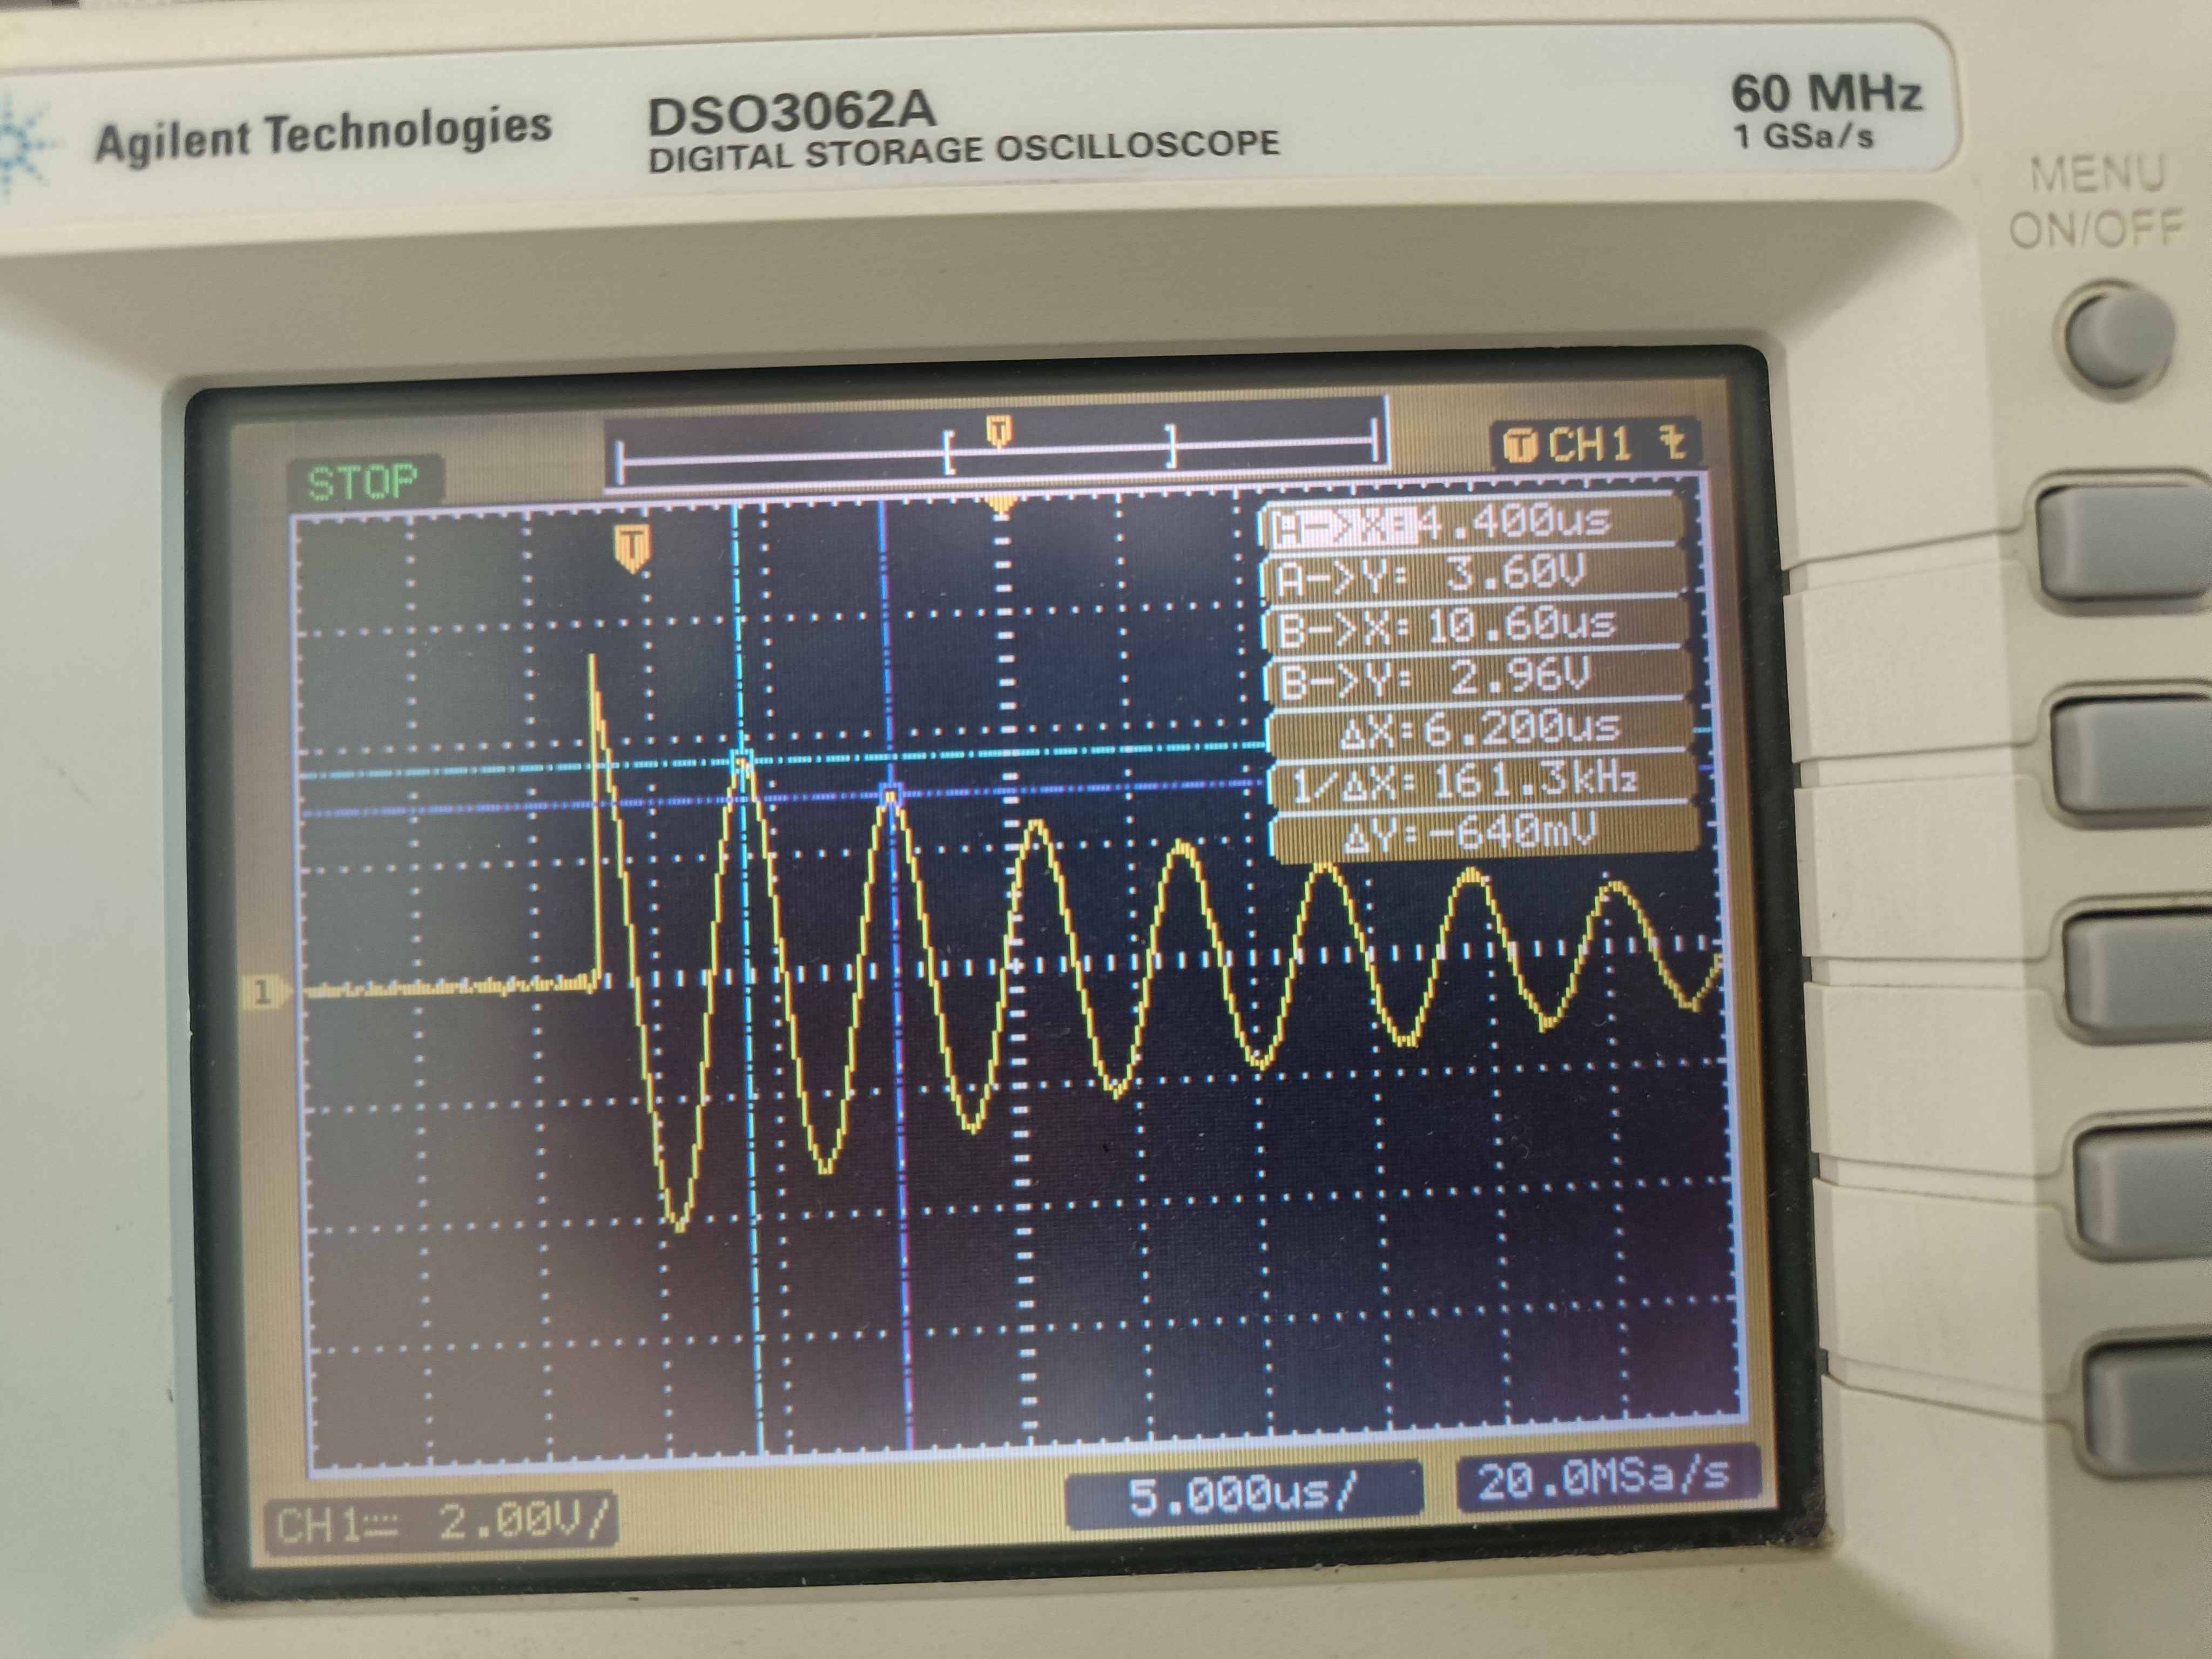
\includegraphics[width=0.7\columnwidth]{pics/560pF.jpg}
	\caption{Transient Response of LC[$L = 2.2mH, C=560pF$]}
\end{figure}

Above reading is across the inductor. Taking reading across the capacitor was impractical as it discharded quick before the oscillation could begin.
From the observation,

\begin{align*}
    T &= 6.2\mu s\\
    \omega &= \frac{2\pi}{T} = 1.013 \times 10^{6} rad/s\\
\end{align*}

We know that, 
\begin{align*}
	\omega < \omega_n
\end{align*}

Thus, we assume $\omega_n$ takes values from $1.013\times10^6$ to $1.143\times10^6 rads/s$

Damping ratio is given by,

\begin{align*}
    \xi &= \sqrt{1- \brak{\frac{\omega}{\omega_n}}^2}\\
    \xi_{max} &= 0.4631
\end{align*}

We can observe that damping ratio is less than 1, implying it is underdamped

The internal resistance in the circuit is given by,
\begin{align*}
    R_{max} &= 2\xi_{max}\sqrt{\frac{L}{C}}\\
    R_{max} &= 2.038 k\Omega
\end{align*}

To find the exact value of $R$, we can use the peak value. From the observation,

\begin{align*}
	V(t=T) &= V_0e^{-\alpha T}\\
	V_0e^{-\alpha T} &= 680 mV\\
	\alpha &= 5.2984\times10^{4} rad/s\\
	R &= 233 \Omega
\end{align*}

\section{Precautions}

\begin{enumerate}
	\item Make sure not to accidentally discharge the capacitor
	\item Make sure the DC generator is connected to ground properly
	\item Use a push button for shorting the inductor and capacitor
	\item Repeat the experiment multiple times to be sure of the reading as it is a sensitive measurement
\end{enumerate}

\end{document}